\newcommand{\letitle}{}
\newcommand{\leauthor}{}

\documentclass[a4paper,10pt]{article}
\usepackage[utf8]{inputenc}
\usepackage{amssymb}
\usepackage{amsmath}
\usepackage{xcolor}
\usepackage{enumitem}
%\usepackage{lstlisting}%
\usepackage[margin=3cm]{geometry}
%\usepackage{stmaryrd}%
\usepackage{bbold}
\usepackage[xcolor,leftbars]{changebar}

\newenvironment{myindentpar}
 {\begin{list}{}
         {\setlength{\leftmargin}{1em}}
         \item[]
 }
 { \end{list}}

\newsavebox{\mybox}
\newlength{\mydepth}
\newlength{\myheight}
\newenvironment{answer}%
{\par\begin{lrbox}{\mybox}\quad\begin{minipage}{\linewidth}\color{black}\setlength{\parskip}{10pt plus 1pt minus 1pt}\vspace*{-.7\baselineskip}}%
{\end{minipage}\end{lrbox}%
\settodepth{\mydepth}{\usebox{\mybox}}%
\settoheight{\myheight}{\usebox{\mybox}}%
\addtolength{\myheight}{\mydepth}%
\noindent\makebox[0pt]{%
  \color{gray}\hspace{-0pt}\rule[-\mydepth]{1pt}{\myheight}}%
  \usebox{\mybox}%
  }

\usepackage{tikz}
\usepackage{pgfplots}
\pgfplotsset{compat=1.15}
\usepackage{mathrsfs}
\usetikzlibrary{arrows}
\usepackage{hyperref}
\setlength{\parskip}{0.15cm}
\hypersetup{
    colorlinks=true,
    linkcolor=blue,
    filecolor=blue,      
    urlcolor=blue,
}

\urlstyle{same}

\everymath{\displaystyle}
\title{\letitle}
\author{\leauthor}
\date{}
\begin{document}
    \section{TIPE Sur la vérification de preuve et la preuve automatique d'appartenance d'un mot à une grammaire.}

\section{Définitions}

\subsection{Les grammaires non contextuelles}

Une grammaire non contextuelle est un quadruplet $G = (T,N_t,S,D)$ où :

\begin{itemize}
\item $T$ est l'alphabet des terminaux
\item $N_t$ est l'alphabet des non terminaux
\item $S \in N_t$ est l'axiome
\item $D$, un ensemble d'éléments de $(N_t \cup T)^\star \times (N_t \cup T)^\star$, est l'ensemble des règles de dérivation.
\end{itemize}

Soit $\rightarrow$ la relation binaire définie sur $(N_t \cup T)^\star$ par
\begin{equation}
\forall m,m' \in (N_t \cup T)^\star, m \rightarrow m' \iff \exists (a,b) \in D, u,v \in (N_t \cup T)^\star / m = uav \text{ et } m' = ubv
\end{equation}
On note $\overset{*}{\rightarrow}$ la cloture transitive et réflexive de $\rightarrow$.\\
Pour $x \in (N_t \cup T)^\star$, notons

$\delta(x) := \{y \in (N_t \cup T)^\star / x \overset{*}{\rightarrow} y\}$
et 

$\eta(x) := \delta(x) \cap T^\star$.

Alors le langage de la grammaire G est le suivant :
\begin{equation*}\mathcal{L} (G) := \eta(S)\end{equation*}

Nous allons supposer que $N_t$ est dénombrable et $T$ est fini.

En OCaml :
\begin{verbatim}
type 'e caractere = T of 'e | Nt of int

type 'a reglec = ('a list) * ('a list);;

type 'e csg = {
    terminaux : 'e array ;
    nonterminaux : 'e array ;
    axiome : 'e caractere ;
    reglesc : ('e caractere) reglec array 
};;
\end{verbatim}
\subsection{Les grammaires contextuelles}

\textbf{  Définition : } Une grammaire non contextuelle est une grammaire $G = (T,N_t,S,D)$ telle que :
\begin{equation*} \forall (a,b) \in D, a \in N_t  \end{equation*}


\begin{verbatim}
type 'a reglenc = ('a list) * ('a list);;

type 'e cfg = {
    terminaux : 'e array ;
    nonterminaux : 'e array ;
    axiome : 'e caractere ;
    reglesnc : ('e caractere) reglenc array 
};;
\end{verbatim}

\textbf{ Exemple : } la grammaire des expressions arithmétiques suffixes.
\begin{align*}
D = &\{(S,SS+)_1,(S,SS*)_2,(S,"N")_3\}\\
\cup&\{(N,C)_4 | (N,NC)_5\}\\
\cup&\{(C,0)_6 | (C,1)_7\}
\end{align*}
(les indices dessus correspondent à une énumération des règles de dérivation, par exemple, $D_5 = (N,NC)$)

\subsection{Fôret de dérivation}

Ici, $G = (T,N_t,S,D)$ est une grammaire non contextuelle.

Une forêt est une liste d'arbres
\begin{verbatim}
type 'a arbre = 'a * 'a foret and
type 'a foret = 'a arbre list
\end{verbatim}


Une preuve qu'un mot appartient à $\eta(m)$ peut être donnée par une forêt de dérivation :

\begin{answer} 
Si $m$ est le mot vide, il s'agit de la forêt vide.

Sinon, soit $n = |m|$,\\
\begin{answer} 
    Si $n=1$, il s'agit d'un seul arbre où la racine est $m$ et chaque sous arbres est la forêt de dérivation d'un $b$ tel que $(m,b) \in D$.

    Si $n>1$, il s'agit de la liste des arbres $[f_1, \dots, f_n]$ où $\forall i \in [1,n], f_i$ est un arbre de dérivation de la lettre $m_i$.
\end{answer}
\end{answer}

\begin{verbatim}
let test_foret_deriv f m gram = match m with
    |[] -> f = []
    |[x] -> 
        List.exists 
        (fun (a,b) -> x = a && test_foret_deriv f b gram) 
        gram.reglesnc
    |t1::q1 -> 
        match f with
            |[] -> false
            |t2::q2 -> (test_foret_deriv [t2] [t1]) && (test_foret_deriv q2 q1)
\end{verbatim}


L'ensemble des forêts de dérivation de $m$ est noté $\mathcal{F}(m)$.

\begin{verbatim}
type 'e caractere = T of 'e | Nt of int
\end{verbatim}

Le parcours infixe des feuilles d'une forêt de dérivation de $x$ donne un mot de $\eta(x)$.
Un exemple sera donnée dans le cas d'une grammaire non contextuelle.

Pour $a \in \mathcal{F}(x)$, on note $\mathcal{I}(a)$ le parcours infixe des feuilles de $a$. 

\subsection{Exemple de preuve}

Une preuve que "10""11"+"0"* $\in \mathcal{L}(G)$ :\\
Lemme 1 : "10" $\in \eta(S)$

    En effet, $S\rightarrow_3 "N" \rightarrow_5 "NC" \rightarrow_6 "N0" \rightarrow_4 "C0" \rightarrow_7 "10"$


L'abre de dérivation fait aussi office de preuve, bien plus concise :
   
\begin{tikzpicture}[level distance=20pt]
    \node {S}
child { node {"} }
child {
    node {N}
    child {
        node {N}
        child {
            node {C}
            child {
                node {1}
            }
        }
    }
    child {
        node {C}
        child {
            node {0}
        }
    }
}
child { node {"} }

    ;
\end{tikzpicture}
    

Lemme 2 : "11" $\in \eta(S)$
Preuve avec l'arbre suivant
 
\begin{tikzpicture}[level distance=20pt]
    \node {S}
child { node {"} }
child {
    node {N}
    child {
        node {N}
        child {
            node {C}
            child {
                node {1}
            }
        }
    }
    child {
        node {C}
        child {
            node {1}
        }
    }
}
child { node {"} }

    ;
\end{tikzpicture}
    

On peut alors, en combinant les deux arbres précédants, prouver que "10""11"+ $\in \eta(S)$ :
 
\begin{tikzpicture}[level distance=20pt]
    \tikzstyle{level 1}=[sibling distance=30mm]
\tikzstyle{level 2}=[sibling distance=10mm] 
\node {S}
child {
    node {S}
    child { node {"} }
    child {
        node {N}
        child {
            node {N}
            child {
                node {C}
                child {
                    node {1}
                }
            }
        }
        child {
            node {C}
            child {
                node {0}
            }
        }
    }
    child { node {"} }
}
child {
    node {S}
    child { node {"} }
    child {
        node {N}
        child {
            node {N}
            child {
                node {C}
                child {
                    node {1}
                }
            }
        }
        child {
            node {C}
            child {
                node {1}
            }
        }
    }
child { node {"} }
}
child {node {+}}
    ;
\end{tikzpicture}
    

Avec l'arbre suivant, on prouve enfin que "10""11"+"0"* $\in \delta(S) \cap T^\star = \mathcal{L}(G)$ :
 
\begin{tikzpicture}[level distance=20pt]
    \tikzstyle{level 1}=[sibling distance=40mm]
\tikzstyle{level 2}=[sibling distance=15mm]
\tikzstyle{level 3}=[sibling distance=5mm]
\node {S}
child {
    node {S}
    child {
        node {S}
        child { node {"} }
        child {
            node {N}
            child {
                node {N}
                child {
                    node {C}
                    child {
                        node {1}
                    }
                }
            }
            child {
                node {C}
                child {
                    node {0}
                }
            }
        }
        child { node {"} }
    }
    child {
        node {S}
        child { node {"} }
        child {
            node {N}
            child {
                node {N}
                child {
                    node {C}
                    child {
                        node {1}
                    }
                }
            }
            child {
                node {C}
                child {
                    node {1}
                }
            }
        }
    child { node {"} }
    }
    child {node {+}}
}
child {
    node {S}
    child {node {"}}
    child {
        node {N}
        child {
            node {C}
            child {
                node {0}
            }
        }
    }
    child {node {"}}
}
child {
    node {*}
}
    ;
\end{tikzpicture}
    

On remarque bien qu'un parcours infixe des feuilles de l'arbre donne "10""11"+"0"*

\section{Vérification de preuve pour une grammaire non contextuelle}

La forêt de dérivation nous donne une bonne manière de vérifier une preuve, car une preuve est caractérisé par une forêt de dérivation.\\

(en pratique, 'e sera string).

Par induction on peut montrer $m \in \eta(x) \iff $ il existe $p$ une forêt de dérivation dont le parcours infixe des feuilles est $m$ et les racines sont les lettres de $x$. 

\begin{answer} 
$
m \in \eta(x)\\
\iff \exists n \in \mathbb{N} / \exists m_1,m_2,\dots,m_n \in (N_t \cup T)^\star / x \rightarrow m_1 \rightarrow m_2 \rightarrow \dots \rightarrow m_n\text{ et }m_n \in T^\star$    $ (2_n)\\
\mathcal{P}(n) := ((2_n) \implies \exists A \in \mathcal{F}(x) / \mathcal{I}(x) = m)$\\
\begin{answer} 
$\mathcal{P}(0) : x \in \eta(x) \implies x \in T^\star$ donc $[B (x_1);\dots;B (x_{|x|})]$ convient.\\
$\forall n \in \mathbb{N}^*,\mathcal{P}(n-1) \implies (m \in \eta(m_1) \implies \exists A \in \mathcal{F}(m_1)/ \mathcal{I}(A) = m)$

 et comme $x\rightarrow m_1,\exists (a,b) \in D, u,v\in (N_t\cup T)^\star /x = uav$ et $m_1 = ubv$

 Soit $p := |u|, q := |v|, r := |b|$
 
 alors $A|_{[1,p]} \in \mathcal{F}(u), A|_{[p+1,p+r]} \in \mathcal{F}(b), A|_{[p+r+1,p+r+q]} \in \mathcal{F}(v)$

 Donc $A|_{[1,p]}@A'@A|_{[p+r+1,p+r+q]}\in \mathcal{F}(x)$ où $A' = N (b,A|_{[p+1,p+r]})$

 Soit $\mathcal{P}(n)$.
\end{answer}
\end{answer}
La réciproque se montre avec un algorithme qui à un arbre de dérivation associe une séquence $m_1,m_2,\dots,m_n \in (N_t \cup T)^\star$ telle que $x \rightarrow m_1 \rightarrow m_2 \rightarrow \dots \rightarrow m_n$

En entrée, nous avons $f_0$, une forêt de dérivation.
\begin{answer} 
$f$ est une copie de $f_0$. 

Tant que $f$ n'est pas constituée que de feuilles :

\begin{answer} 
    On prend $a$ un arbre qui n'est pas une feuille dans $f_0$

    Remplacer $a$, dans $f$, par ses fils.

    Lire les racines de la forêt de gauche à droite.
\end{answer}
\end{answer}
En remplaçant $a$ dans $f$ par ses fils, on dérive notre mot une fois.\\\\

\fbox{Alors $a \in \mathcal{F}(S)$ est une preuve que $\mathcal{I}(a) \in \mathcal{L}(G)$.}

Alors, vérifier une preuve donnée par une forêt consiste juste à vérifier que la forêt est bien une forêt de dérivation.

\section{Preuve automatique en grammaire non contextuelle}

Toujours dans une grammaire non contextuelle

Avec une grammaire dont l'axiome est S,
pour générer automatiquement une preuve, l'idée est qu'à chaque étape,
on dispose d'une liste de mots prouvés,
et à chaque étape, on fait toutes les dérivations possibles de notre liste de mots prouvés pour obtenir une liste de mots prouvés plus grande.

Deux approches coexistent alors, soit on fait toutes les dérivations possibles dans le sens direct, soit dans le sens indirect.

\subsection{La méthode bottom-up}

On part des $\left\{ [B(b_1);\dots;B(b_n)] | (a,b)\in D \text{ et } b \in T^\star , n = |b|\right\}$ et on construit d'autres arbres de dérivation à partir des règles de dérivation.

Par la méthode bottom-up, on générerait dans l'ordre :\\
à l'étape 0 :
 
\begin{tikzpicture}[level distance=20pt]
    \draw (0,0) node {0};
\draw (1,0) node {1};
    ;
\end{tikzpicture}
    
à l'étape 1 : 
 
\begin{tikzpicture}[level distance=20pt]
    \draw (0,0) node {C}
child {
    node {0}
};

\draw (1,0) node {C}
child {
    node {1}
};

\draw (2,0) node {0};

\draw (3,0) node {1};
    ;
\end{tikzpicture}
    
à l'étape 2 : 
 
\begin{tikzpicture}[level distance=20pt]
    \draw (0,0) node {N}
child {
    node {C}
    child {
        node {0}
    }
};

\draw (1,0) node {N}
child {
    node {C}
    child {
        node {1}
    }
};

\draw (2,0) node {C}
child {
    node {0}
};

\draw (3,0) node {C}
child {
    node {1}
};

\draw (4,0) node {0};

\draw (5,0) node {1};
    ;
\end{tikzpicture}
    
à l'étape 3 : 
 
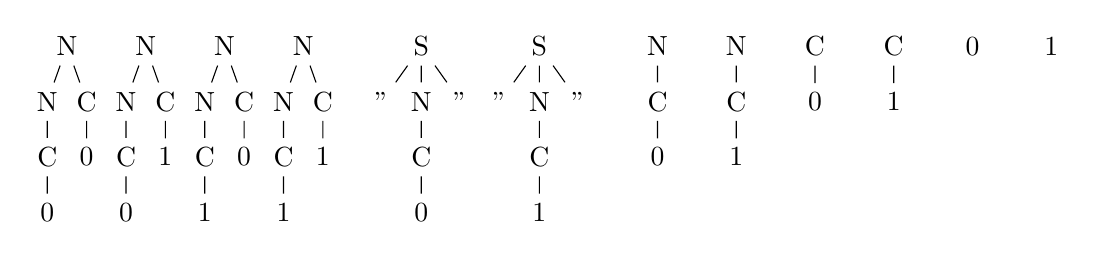
\begin{tikzpicture}[level distance=20pt]
    \tikzstyle{level 1}=[sibling distance=5mm]
\draw (0,0) node {N}
child {
    node {N}
    child {
        node {C}
        child {
            node {0}
        }
    }
}
child {
    node {C}
    child {
        node {0}
    }
};

\draw (1,0) node {N}
child {
    node {N}
    child {
        node {C}
        child {
            node {0}
        }
    }
}
child {
    node {C}
    child {
        node {1}
    }
};

\draw (2,0) node {N}
child {
    node {N}
    child {
        node {C}
        child {
            node {1}
        }
    }
}
child {
    node {C}
    child {
        node {0}
    }
};

\draw (3,0) node {N}
child {
    node {N}
    child {
        node {C}
        child {
            node {1}
        }
    }
}
child {
    node {C}
    child {
        node {1}
    }
};

\draw (4.5,0) node {S}
child {
    node {"}
}
child {
    node {N}
    child {
        node {C}
        child {
            node {0}
        }
    }
}
child {
    node {"}
};

\draw (6,0) node {S}
child {
    node {"}
}
child {
    node {N}
    child {
        node {C}
        child {
            node {1}
        }
    }
}
child {
    node {"}
};

\draw (7.5,0) node {N}
child {
    node {C}
    child {
        node {0}
    }
};

\draw (8.5,0) node {N}
child {
    node {C}
    child {
        node {1}
    }
};

\draw (9.5,0) node {C}
child {
    node {0}
};

\draw (10.5,0) node {C}
child {
    node {1}
};

\draw (11.5,0) node {0};

\draw (12.5,0) node {1};
    ;
\end{tikzpicture}
    

On prouve par induction simple qu'à l'étape $k$, on a généré tous les arbres de dérivations possibles de profondeur $k$.

\subsection{La méthode top-down}

On part de l'axiome $S$ de la grammaire pour construire des mots de $\delta(S)$ en remplaçant un nonterminal $x$ d'un mot par un $b$ d'une règle de dérivation $(x,b)$.

Cette méthode suit d'assez près la définition des mots de la grammaire\\
(on peut écrire la clôture transitive et réflexive $\overset{*}{\rightarrow}$ comme :
$\overset{*}{\rightarrow} = \bigcup_{n \in \mathbb{N}} \rightarrow ^n$ où $\rightarrow^k$ est $\rightarrow$ composée $k$ fois).\\
On génère en effet, avec cette méthode, à la $n$-ième étape, $A_n = \left\{m \in (N \cup T)^\star \mid  S \left(\bigcup_{k \in [1,n]} \rightarrow^k\right) m\right\}$.
Il est alors simple de vérifier que tout mot du langage de la grammaire sera généré en temps fini par cette méthode.

On génère alors dans l'ordre :\\
à l'étape 0 : $\{S\}$, \\
à l'étape 1 : $\{S,SS+,SS*,"N"\}$,\\
et à l'étape 2 : $\{S,SS+,SS*,"N",SS*S+,SSS*+,SSS+*,SS+S*,$ \\
$"N"S+,S"N"+,"N"S*,S"N"*,"C","NC"\}$.

Cette méthode est bien plus proche de la définition et est directement applicable aux grammaire contextuelles.

\subsection{En grammaire contextuelle}

Chercher automatiquement une preuve d'appartenance d'un mot à une grammaire non contextuelle se fait déjà très bien avec les automates à pile.
Nous allons ici nous intéresser plus spécifiquement aux grammaires contextuelles, et réutiliser notre méthode top-down.
La méthode s'applique alors directement de la même manière.
Nous avons donc un algorithme qui permet théoriquement de prouver que n'importe quel mot de la grammaire appartient bien à cette dernière.
Le problème étant la complexité de ce dernier, qui fonctionne comme une machine non déterministe où on ne coupe pas les instances arrivant à un état puit.
La suite va donc consister à trouver, de manière heuristique ou non, des méthodes affirmant qu'à partir d'un mot $m$, on aura des difficultés à dériver en notre mot $m'$ à prouver.
Alors, nous allons arrêter les recherches de dérivations de S en $m'$ qui passent par le mot $m$.

\end{document}
    